\chapter{\IfLanguageName{dutch}{Stand van zaken}{State of the art}}
\label{ch:stand-van-zaken}
Eén van de grote voordelen aan een smartphone is dat je altijd en overal toegang hebt tot informatie. Toch kan niet iedereen die voordelen ten volle benutten. Aanpassingen aan mobiele applicaties zijn noodzakelijk om zoveel mogelijk mensen die voordelen ten volle te kunnen laten benutten. De mobiele platformen iOS en Android bieden een uitgebreid assortiment aan functionaliteiten om deze aanpassingen mogelijk te maken. Om een duidelijk beeld te krijgen over het probleemdomein zal dit hoofdstuk analyseren wat de huidige situatie betreffende toegankelijkheid is en wat de verschillende beperkingen en mobiele platformen zijn.

%Om duidelijkheid een duidelijker beeld te scheppen over de huidige situatie rondom toegankelijkheid op mobiele platformen, zal dit hoofdstuk dieper ingaan op 


\section{Toegankelijkheid}
\label{sec:toegankelijkheid}
Toegankelijkheid is misschien voor velen een abstract begrip. Toegankelijkheid is het bruikbaar maken van zowel de gewone wereld als de digitale wereld voor iedereen \autocite{anySurferWat}. In dit onderzoek zal de focus gelegd worden op het toegankelijk maken van de digitale wereld. Meer bepaalt het bruikbaar maken van mobiele applicaties. Want mobiele applicaties bieden ons net als websites toegang tot communicatie, informatie, educatie en nog zoveel meer  \autocite{introAccesibilityw3c}. Toegankelijkheid in de digitale wereld wordt steeds belangrijker, de digitale revolutie zorgt ervoor dat steeds meer informatie voornamelijk digitaal wordt overgebracht. Mensen met een beperking hebben nood aan toegankelijkheid en slagen er niet altijd in om informatie op de daarvoor voorziene manier te verkrijgen. Er zijn aanpassingen nodig om die doelgroep ook toegang te bieden aan die informatie. Wanneer de digitale wereld er niet in slaagt om hun mobiele applicaties toegankelijker te maken dreigt er een grote doelgroep uit de boot te vallen.







\subsection{Wetgeving}
\label{sec:wetgeving}
Dankzij wettelijke bepalingen zal in sommige gevallen de ontwikkelaars verplicht worden om
hun applicaties toegankelijker te maken. Want toegankelijkheid zorgt ervoor dat mensen
met een beperking ook kunnen functioneren in onze maatschappij. Door deze wetgevingen probeert men ontwikkelaars ervan te behoeden om deze specifieke doelgroep te vergeten.
Door de geschiedenis heen zijn er verschillende verdragen en wettelijke bepalingen vastgelegd.
De belangrijkste worden hieronder besproken.

\subsubsection{Verdrag inzake rechten van personen met een handicap}
\label{vn-Verdrag}
Het verdrag die op 13 december 2006 door de Verenigde Naties (VN) goedgekeurd is, heeft als essentie dat mensen met een beperking evenveel rechten hebben als iemand anders en daarbij ook ondersteund moeten worden om deze rechten te bekomen. Het VN-Comité kijkt er dan ook op toe dat het verdrag gerespecteerd wordt. Niet voldoen aan deze richtlijnen kan worden gezien als het discrimineren van een individu \autocite{unia2006}. 

Binnen de contouren van dit onderzoek is voornamelijk \textbf{artikel 9} van belang. Dit artikel beschrijft hoe de ondertekende landen mensen met een beperkingen moeten faciliteren zodat ze beter kunnen functioneren in de samenleving. Hieronder valt onder andere betere toegang tot informatie, toegang tot communicatie, toegang tot nieuwe technologieën, etc..  \autocite{un2006}

%Nog iets over belgie hier?
\subsubsection{The European Accessibility Act}
De Europese Commissie wil met de European Accessibility Act (EAA) de ongeveer 80
miljoen mensen met een beperking volledige en gelijke participatie in de gemeenschap
garanderen.


Binnen verschillende lidstaten van Europa werd het verdrag van de Verenigde Naties
(VN) geïmplementeerd met elk zijn eigen regelgeving omtrent toegankelijkheid. Handel
van producten en diensten met aanpassingen voor toegankelijkheid tussen verschillende
lidstaten verloopt moeizaam en dit doordat elke lidstaat een specifieke regelgeving heeft.
Dit zorgt voor een barrière voor het implementeren van aanpassingen bij producten die
verhandeld worden in meerdere lidstaten.


De EAA is bedoeld om in alle lidstaten binnen Europa dezelfde functionele vereisten te
stellen aan producten en diensten. Met als doel toegankelijkheid makkelijker implementeerbaar te maken en met het voordeel dat mensen met een
beperking toegankelijkere producten hebben en bedrijven in elke lidstaat dezelfde set van
vereisten hebben.


Lidstaten worden verplicht de EAA te implementeren. Maar voldoen bij het succesvol
implementeren ook aan het verdrag opgesteld door de VN
 \autocite{eaa2015}.



\subsubsection{Directive (EU) 2016/2102}
\label{directive}
De richtlijn 2016/2102 van het Europese parlement van 26 oktober 2016 richt zich op het
verhogen van de toegankelijkheid van digitale informatie afkomstig van overheidsinstanties.
Deze richtlijn benadrukt het belang van toegankelijkheid voornamelijk omdat de digitale maatschappij zich steeds meer ontwikkelt en de ’digitale agenda’ van Europa die online content probeert te bevorderen steeds meer uitrolt. De informatie die beschikbaar wordt gesteld door overheden, die trouwens een voorbeeldfunctie hebben, moet dus op een niet discriminerende manier beschikbaar gesteld worden.


 Zowel websites als mobiele applicaties van overheidsinstanties moeten voldoen aan de toegankelijkheidseisen die voorop gesteld worden. Verschillende lidstaten hebben zelf een invulling gegeven aan toegankelijkheidseisen. Toch wil deze richtlijn een aantal gemeenschappelijke eisen voor alle lidstaten opleggen. Dit zorgt ervoor dat ontwikkelaars en ontwerpers minder obstakels hebben en kosten kunnen dalen op gebied van toegankelijkheid.

De richtlijn stelt ook dat indien mogelijk alle content/informatie toegankelijk zou moeten zijn en anders moet er een toegankelijk alternatief zijn. Websites en mobiele applicaties van overheidsinstanties moeten dus op de eerste plaats waarneembaar, bedienbaar, begrijpelijk en robuust gemaakt worden.
 
Er wordt verwacht van de lidstaten dat mobiele applicaties van overheidsinstanties voldoen aan deze richtlijn tegen 23 juni 2021 \autocite{directive2016}.

\subsection{W3C WAI toegankelijkheid standaarden/richtlijnen}
\label{sec:standaarden}
De W3C (World Wide Web Consortium) is een organisatie die standaarden probeert voor te schrijven voor het web. Een onderdeel van deze organisatie is het W3C Web Accessibility Initiative (WAI), zij hebben als doel het toegankelijker maken van het web
 \autocite{introAccesibilityw3c}. De standaarden beschreven door W3C omtrent toegankelijkheid worden gezien als internationale standaarden en zijn ook het vertrekpunt voor de diverse Europese normen en richtlijnen.
 
De W3C WAI zijn vooral gericht op webapplicaties en web pagina's, toch kunnen de richtlijnen \textbf{WCAG 2.1} toegepast worden op alle soorten mobiele applicaties. Dit komt doordat vaak de user interface van mobiele applicaties vergelijkbaar is met web applicaties. Toch bieden mobiele applicaties een groot aantal toegankelijkheidstekorten die anders zijn dan web applicaties \autocite{w3mobileConsider}. Dit onderzoek baseert zich grotendeels op deze richtlijnen omdat deze van een internationale standaard zijn.

Het is belangrijk te weten dat er geen aparte richtlijnen voor mobiele applicaties zijn, deze zijn allemaal opgenomen in de WCAG richtlijnen. \textbf{WCAG 2.1} gepubliceerd in juni 2018 bevat wel extra criteria gericht op mobiele applicaties.
\autocite{w3cMobileGuidelines}

\subsection{Doelgroep}
\label{sec:doelgroep}

Het grootste deel van de mensen die nood hebben aan het toegankelijker maken van mobiele applicaties zijn mensen met een beperking. Uit cijfers van \textcite{who2018} blijkt dat ongeveer 15\% van de wereldpopulatie in één of andere vorm een beperking heeft. Dit is een grote groep, die zeer waarschijnlijk ook gebruikmaken van mobiele applicaties. Dit is een grote groep die hoogst waarschijnlijk ook gebruikmaken van mobiele applicaties. Deze groep zijn permanent beperkt. De redenen waarom aanpassingen nodig zijn voor mensen met een beperking zijn heel divers. De verschillende beperkingen worden verder in dit hoofdstuk besproken. 

Senioren behoren ook tot onze doelgroep aangezien zij te kampen krijgen met ouderdomsverschijnselen en die zorgen er voor dat ze ook beperkt kunnen zijn in hun dagelijks functioneren. Het onderzoek van \textcite{diaz2014accessibility} bevestigt dat er aandacht moet besteed worden aan de oudere generatie om uitsluiting te voorkomen.  Aanpassingen voor senioren zou hun ook meer stimuleren om technologie te gebruiken.


Aanpassingen doorvoeren op maat van senioren zou er ook voor kunnen zorgen dat deze mensen zich makkelijker wagen aan de digitale wereld. Een ander belangrijk aandeel zijn mensen zonder beperkingen. Hieronder vallen mensen met een tijdelijke beperking, bijvoorbeeld een gebroken arm. Maar ook diegene met een situatie beperking, bijvoorbeeld dronken zijn \autocite{inclusiveMicrosoft}. Voor zowel tijdelijke als situatie beperkingen kunnen aanpassingen zeer welkom zijn. Een voorbeeld hiervan is het gebruik van spraakbesturing wanneer men aan het autorijden is. Zie figuur \ref{fig:personaSpect} voor een visualisatie van tijdelijke en situatie beperkingen.

\begin{figure}[h]
    \centering
    \label{fig:personaSpect}
    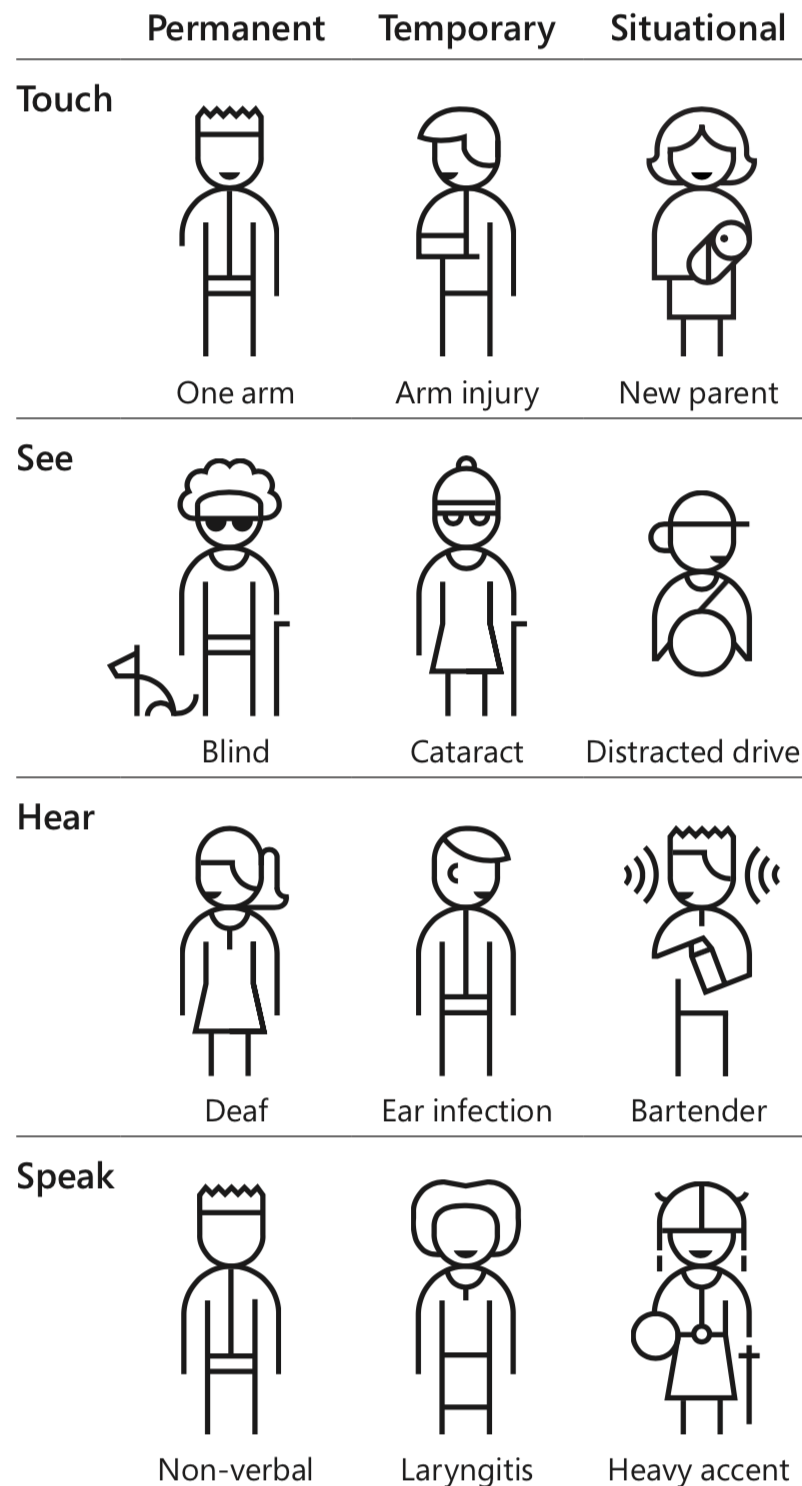
\includegraphics[width=0.3\linewidth]{img/doelgroep_situatie_tijdelijk}
    \caption{Persona spectrum \autocite{inclusiveMicrosoft}}
\end{figure}





\section{Beperkingen}
\label{sec:beperkingen}
Om een beter inzicht te krijgen hoe toegankelijkheid verhoogd kan worden is ook kennis over de verschillende beperkingen essentieel. Er zijn veel verschillende beperkingen, in dit onderzoek worden ze per type gegroepeerd. Deze types zijn vernoemd naar de functie die beperkt wordt. De verschillende domeinen in beperkingen die behandeld worden in dit onderzoek zijn respectievelijk:
\begin{itemize}
    \item Visueel
    \item Auditief
     \item Motorisch
     \item Cognitief
    \end{itemize}


De term beperking beschrijft het gelimiteerd zijn in uitvoeren van activiteiten of het hebben van bepaalde restricties. \autocite{whoDis2019}. Dit door het beperkt zijn in het uitvoeren van bepaalde lichaamsfuncties en dit op een tijdelijke of permanente basis. Vaak is ook ondersteuning nodig om te kunnen functioneren zoals dat wenselijk is.

\subsection{Visueel}
\label{sec:Visueel}
Een zeer belangrijke lichaamsfunctie is het zicht, dankzij dit zintuig kunnen er verschillende prikkels waargenomen worden. Toch is niet iedereen instaat om op een normale manier deze prikkels waar te nemen. Het zicht kan beperkt zijn, waarbij dat ook nog sterk kan variëren in sterkte en oog. Dit op tijdelijke of permanente tijdsbasis \autocite{accessibility2019}.

\subsubsection{Kleurenblindheid}
Iemand die kleurenblind is die ziet nog kleuren maar niet op een correcte manier. De meeste mensen worden met kleurenblindheid geboren maar kan ook veroorzaakt worden door ziekten. 
Het type kleurenblindheid dat het meeste voorkomt is rood-groen stoornis.  Ongeveer 8,00\% van de mannen en 0,04\% van de vrouwen lijden aan deze stoornis. 

Onze lichtgevoelige cellen in ons netvlies zijn verantwoordelijk voor omzetting van kleur naar onze hersenen. Door het niet goed functioneren van enkele van die cellen ontstaat er kleurenblindheid. De cellen verantwoordelijk voor die omzetting van kleur worden ook wel kegeltjes genoemd. Een defect in de hersenen kan ook een oorzaak zijn voor kleurenblindheid. Figuur \ref{fig:ballenbak} toont 3 belangrijke soorten kleurenblindheid. Ze hebben de volgende kenmerken: 
\begin{itemize}
    \item \textbf{Protanoop}: rode kleur waarneming verstoort.
    \item \textbf{Deuteranoop}: groene kleur waarneming verstoort.
    \item \textbf{Tritanoop}: blauwe kleur waarneming verstoort.
\end{itemize}
Het verschil in de soorten kleurenblindheid ligt in het aantal en soort kegeltjes die niet correct functioneren \autocite{visioKleur2019}.



\begin{figure}[!h]
    \centering
    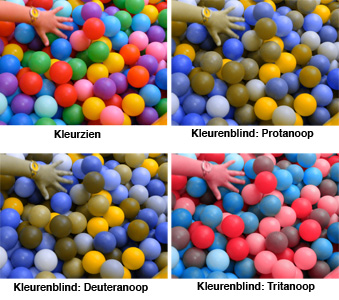
\includegraphics[width=0.5\linewidth]{img/ballenbak}
    \caption{Visuele voorstelling soorten kleurenblindheden \autocite{visioKleur2019}.}
    \label{fig:ballenbak}
\end{figure}



\subsubsection{Slechtziend en blindheid}
Men spreekt van slechtziendheid wanneer het gezichtsvermogen sterk is verminderd en dit niet oplosbaar is. Er wordt gesproken van zwaar slechtziendheid wanneer men een gezichtsscherpte heeft van maximaal 30,00\% of een klein gezichtsveld heeft die kleiner of gelijk is aan 20 graden. Er bestaan heel veel soorten slechtziendheid. Zo kan iemand heel wazig zicht hebben door een zwakke gezichtsscherpte of tunnelzicht door een klein gezichtsveld.

 Er wordt gesproken van blindheid wanneer men maar maximaal 5,00\% gezichtsscherpte meer bezit. Dit betekent dat men nog zicht heeft maar heel beperkt. Ook wanneer men een gezichtsveld heeft van maximaal 10 graden spreekt men van blindheid \autocite{LiLi2019Blind}.




\subsubsection{Verhogen toegankelijkheid}
Bij slechtziendheid of blindheid wordt er vaak gefocust op de andere zintuigen zoals tastzin of het gehoor. In smartphones zal men dan voornamelijk gebruik maken van geluid om de toegankelijkheid te verhogen. Kleurenblindheid kan worden ondersteund door het contrast van gebruikte kleuren te verhogen of zelfs de kleuren benoemen helpt bij het gebruik van een smartphone \autocite{visioKleur2019}.


\subsection{Auditief}
\label{sec:Auditief}

Een ander belangrijk zintuig is het gehoor. Het laat ons ook toe om prikkels van geluid op te nemen. Mensen met een auditieve beperking hebben moeite met het waarnemen van deze prikkels. Dit kan zich uiten in het slechthorend zijn of zelfs doof zijn. Ongeveer 5\% van de wereldpopulatie lijdt aan een auditieve beperking \autocite{whoDAHL2019}.

\subsubsection{Slechthorend en doof}
Wanneer men niet in staat is waar te nemen wat een persoon met normaal gehoor kan waarnemen wordt gezien als slechthorend. Slechthorendheid kan voorkomen in één oor of beide oren. Men spreekt van slechthorendheid wanneer men in een volwassen oor een verlies van meer dan 40 decibel heeft, in een kinderoor een verlies van meer dan 30 decibel vergeleken met een goed horend persoon. Het beperkt een persoon in het normaal communiceren met anderen omdat er moeite is met het waarnemen van het gesprek \autocite{whoDAHL2019}.


  Doofheid is de toestand waarbij men aan een groot gehoorverlies lijdt die vaak onherstelbaar is. In dit geval moet gezocht worden naar alternatieve manieren voor te communiceren \autocite{accessibility2019}.

\subsubsection{Verhogen toegankelijkheid}
Voor het vervangen van audio bij het gebruik van mobiele applicaties kan men gebruik maken van tekst. Het ondertitelen, of transcripten van audio verhoogt de toegankelijkheid voor blinden en slechtzienden \autocite{accessibility2019}.

\subsection{Motorisch}
\label{sec:Motorisch}
Een motorische beperking, ook wel fysieke beperking genoemd, is een toestand wanneer iemand een beperkte fysieke capaciteit heeft en/of minder mobiel is. Bewegingen gaan hierdoor moeizamer dan anders. Een motorische beperking kan aangeboren zijn maar kan ook veroorzaakt zijn door een ziekte of een ongeval  \autocite{achieveAU2019}.

\subsubsection{Verhogen toegankelijkheid}
Er zijn verschillende soorten beperkingen waarbij ofwel geen handfunctie meer is of die heel er verstoord is door bijvoorbeeld ongewenste bewegingen. Wanneer men hier last van heeft kan het bedienen van een smartphone een grote uitdaging zijn. Kleine klikgebieden vervangen door grotere oppervlakten, voldoende tijd geven voor het uitvoeren van taken en nog veel meer kan mensen met deze beperking ondersteunen bij hun smartphone gebruik  \autocite{accessibility2019}.







\subsection{Cognitief}
\label{sec:cognitief}
Cognitieve beperkingen zijn beperkingen die zorgen voor mentale, leer en/of psychologische beperkingen. Onder de term cognitief beperkt vallen vele verschillende soorten limiteringen. Dit onderzoek beperkt zich tot:
\begin{itemize}
    \item Gedragsstoornissen
    \item Neurologische stoornissen 
\end{itemize}

Er bestaan een groot aantal gedragsstoornissen maar bij het gebruik van een smartphone gaan personen met ADHD (Attention Defict Hyperactivity Disorder) of mensen met ADD (Attention Defict Disorder) vaak moeilijkheden hebben met het concentreren. Autisme
zorgt ervoor dat een individu moeite heeft met communiceren en interactie.


Bij neurologische stoornissen is er vaak een probleem in de hersenen. Epilepsie is een stoornis waarbij mensen zeer gevoelig zijn aan lichtflitsen. Andere voorbeelden van neurologische stoornissen zijn dementie, psychologische problemen, ... 
\autocite{patel2016mental}

\subsubsection{Verhogen toegankelijkheid}
Voor mensen met ADD of ADHD is het wenselijk om zoveel mogelijk afleidingen te voorkomen. Bij autisme moet men zorgen dat er een voorspelbare en eenvoudige inhoud is. Consistentie is ook zeer belangrijk voor mensen met autisme.

Wanneer men te maken heeft met neurologische stoornissen zoals epilepsie moet men vooral het gebruik van lichtflitsen beperken of opties aanbieden om deze te beperken. Het gedrag van de applicatie zo voorspelbaar mogelijk maken en eventueel afbeeldingen gebruiken 
 \autocite{accessibility2019}.



\section{Mobiele platformen}
\label{sec:mobielePlatformen}
De mobiele industrie kende in de afgelopen jaren een enorme groei. Er is geëvolueerd naar een mobiele revolutie waarbij veel informatie altijd en overal beschikbaar is. 

Het is niet de hardware van een smartphone maar de software die het meeste invloed heeft op ons. Dankzij het mobiel platform die op een smartphone draait kan er interactie plaatsvinden. Het laat ons toe om te surfen op het web, applicaties te gebruiken en nog veel meer. Wanneer een mobiel platform toegankelijk genoeg is kunnen mensen met een beperking zeker ook gebruik maken van deze voordelen. 


Uit statistieken van \textcite{statMobile2019} blijkt dat Android een marktaandeel heeft van 74,15\%, iOS volgt daarna met een marktaandeel van 23,28\%. Samen is dit goed voor een marktaandeel van 97,43\%. Er kan aangenomen worden dat Android en iOS een groot genoeg marktaandeel hebben. Deze 2 vallen door dat marktaandeel dan ook binnen de scope van dit onderzoek

Uit de resultaten van een onderzoek van \textcite{webAIMSurvey} valt af te leiden dat het gebruik van toegankelijkheidsvoorzieningen op mobiele apparaten zeer populair is. Op de vraag of er gebruik wordt gemaakt van een screen reader op een mobiel apparaat heeft van de 1770 respondenten 88,00 \%, positief geantwoord. 90,90\% van de respondenten die een beperking heeft gebruikt een screen reader.


Zowel Android en iOS hebben een grote set van functionaliteiten beschikbaar voor het verhogen van de toegankelijkheid. De functionaliteiten die hieronder besproken worden, zijn diegene die de mobiele platformen hebben beschikbaar gesteld voor haar gebruikers. Voor sommige functionaliteiten moeten ontwikkelaars gebruik maken van \gls{API}'s om deze bruikbaar te maken in hun mobiele applicatie. In hoofdstuk x%TODO:Hoofstuk%
 zal een vergelijking gemaakt worden inzake de beschikbare functionaliteiten voor beide platformen, dit zowel op vlak van functionaliteiten beschikbaar voor de gebruiker, als op vlak van \gls{API}'s die beschikbaar zijn.
\\
\\
De verschillende domeinen zullen gedurende deze sectie afgekort worden als:
\begin{itemize}
    \item \textbf{(V)} Visueel 
    \item \textbf{(A)} Auditief 
    \item \textbf{(M)} Motorisch 
    \item \textbf{(C)} Cognitief
\end{itemize} 

Verder kunnen bij bepaalde functionaliteiten gebruikers zonder nood aan toegankelijkheid ook baat hebben. Dit zal aangeduid worden als een \textbf{+}. De functionaliteiten waar alle domeinen van toepassing op zijn wordt aangeduid met een \textbf{*}.
\newpage
\subsection{Android}
\newglossaryentry{API}{name=API,description={Application programming interface}}
\newglossaryentry{Text-to-speech}{name=Text-to-speech ,description={Produceren van gesproken taal uit tekst}}
\newglossaryentry{talkback}{name=Talkback ,description={Talkback geeft audio-feedback wat er op een Android toestel gebeurt, zo kan men het toestel besturen zonder te kijken}}

Doorheen de jaren is het mobiele platform Android sterk gevolueerd, doorheen verschillende versies zijn nieuwe functionaliteiten uitgerold geadresseerd naar het verhogen van de toegankelijkheid. In onderstaande tabel vindt u enkele functionaliteiten en de versie waarbij deze zijn toegevoegd.
\label{sec:Android}

 \begin{table}[h]
   % \usepackage{color}
       \centering
% \usepackage{multirow}
      \caption{Updates Android toegankelijkheid functionaliteiten \autocite{AndroidReleases}.}
    \label{androidUpdates}

    \begin{tabular}{|l|l|l|} 
        \hline
        \textbf{Versienummer} & \textbf{Domein} & \textbf{Toevoegingen/aanpassingen}                \\ 
        \hline
        \multirow{2}{*}{1.6}  & V               & \gls{Text-to-speech}                            \\ 
        \cline{2-3}
        & *               & Eigengemaakte accessibility services               \\ 
        \hline
        \multirow{4}{*}{4.0}  & V               & \gls{talkback}~                                         \\ 
        \cline{2-3}
        & V               & Vergroten lettertype                              \\ 
        \cline{2-3}
        & V               & Screen reader in webbrowser                        \\ 
        \cline{2-3}
        & M               & Touch gebaar voor activatie functionaliteiten     \\ 
        \hline
        4.2                   & V               & Ondersteuning braille-apparaten (Brailleback)     \\ 
        \hline
        4.4                   & A \& +          & Ondertitelingen bij ondersteunde media            \\ 
        \hline
        \multirow{2}{*}{5.0}  & M               & Toegang via schakelaar           \\ 
        \cline{2-3}
        & V               & Kleurenblind filters                              \\ 
         \cline{2-3}
        \hline
        \multirow{5}{*}{7.0}  & *               & Toegankelijkheidsettings beschikbaar vanaf setup  \\ 
        \cline{2-3}
        & A               & Mono-uitvoer geluid                               \\ 
         \cline{2-3}
        & V               & Selecteer voor uitspreken                            \\ 
        \cline{2-3}
        & V               & Aanpasbare snelheid \gls{Text-to-speech}                            \\ 
        \cline{2-3}
        & V \& +          & Schermgrootte aanpassen                           \\ 
        \hline
        \multirow{2}{*}{8.0}  & M~              & Hardware shortcut voor activatie features         \\ 
        \cline{2-3}
        & M               & Gebaren op vingerprintsensor als invoermanier     \\ 
        \hline
        \multirow{5}{*}{9.0}  & *               & Toegankelijkheidsmenu                             \\ 
        \cline{2-3}
        & V               & Voorlezen tekst met camera                        \\ 
        \cline{2-3}
        & C               & Verwijderen animaties                       \\ 
        \cline{2-3}
        & V \& +               & Automatisch roteren scherm optie                       \\ 
        \cline{2-3}
        & A \& +          & Geluidsversterker~                                \\
        \hline
    \end{tabular}

 \end{table}


De functionaliteiten besproken in tabel \ref{androidUpdates} zijn gericht naar de gebruikers. Zoals vermeld in de inleiding van sectie \ref{sec:mobielePlatformen} moeten ontwikkelaars in bepaalde gevallen een inspanning doen om hun applicaties bruikbaar te maken met de bovenstaande functionaliteiten. Bij Android is er ook een \gls{API} beschikbaar voor het maken van eigen toegankelijkheid functionaliteiten voor gebruikers. Dit is geïntroduceerd in versie 1.6 van het mobiele platform. 

Functionaliteiten zoals 'schermgroote aanpassen' en de 'automatisch roteren' optie zijn gericht op personen met een beperking, worden doorgaans vaak gebruikt door de gemiddelde gebruiker. Het zijn aanpassingen die het gebruikersgemak verhogen.
\newpage
\subsection{iOS}
\label{sec:iOS}
% Hier zeker P
% \usepackage{color}

\newglossaryentry{zoom}{name=Zoom,description={Met Zoom kan het scherm op een iOS apparaat ingezoomed worden}}
\newglossaryentry{Begeleide toegang}{name=Begeleide toegang,description={Met begeleide toegang kan op een iOS apparaat bepaalde functies deactiveren}}
\newglossaryentry{Switch_Control}{name=Switch Control,description={Met Switch Control kan op een iOS apparaat bedienen met schakelaar. Dit kan extern zijn, op het scherm, of met de camera van het apparaat}}
\newglossaryentry{Aangepaste_aanraking}{name=Aangepaste aanraking           ,description={Met aangepaste aanrakingen kan op een iOS apparaat de reactie op aanrakingen aangepast worden}}
\newglossaryentry{VoiceOver}{name=VoiceOver,description={Laat toe om een iOS apparaat te besturen op basis van gesproken feedback en gebaren, het wordt ookwel screen reader genoemd}}

% \usepackage{color}
% \usepackage{multirow}

Volgens het onderzoek van \textcite{webAIMSurvey} is iOS het populairst voor het gebruik van mobiele screen readers. Van de 1515 respondenten verkiest 75,60\% iOS. Ze concluderen dat personen die ervaren zijn met screen readers en het internet meer geneigd zijn voor iOS te kiezen. 

iOS laat in vergelijking met Android ontwikkelaars niet toe om functionaliteiten toe te voegen in hun mobiel platform. Wel zet Apple zeer hard in op het toegankelijk maken van iOS. Dit valt vooral te merken in de beschikbare functionaliteiten, de \gls{API}'s die er beschikbaar zijn. Apple is ook zeer bewust bezig met toegankelijkheid te promoten, zowel bij gebruikers als ontwikkelaars. In onderstaande tabel vindt u enkele functionaliteiten en de versie waarbij deze zijn toegevoegd.
\begin{table} [h]
   % \usepackage{multirow}
        \caption{Updates iOS toegankelijkheid functionaliteiten \autocite{appleReleaseNotes}.}
  \label{iOSUpdates}
       \centering
       \begin{tabular}{|l|l|l|} 
           \hline
           \textbf{Versienummer} & \textbf{Domein} & \textbf{Toevoegingen/aanpassingen}          \\ 
           \hline
           \multirow{4}{*}{3.0}  & V               & \gls{VoiceOver}                    \\ 
           \cline{2-3}
           & V               & \gls{zoom}                                        \\ 
           \cline{2-3}
           & V               & Zwart-op-wit voor hoger contrast            \\ 
           \cline{2-3}
           & A               & Mono-uitvoer geluid            \\ 
           \hline
           \multirow{3}{*}{5.0}  & A   \& +             & Ledflits meldingen                          \\ 
           \cline{2-3}
           & A \& +                & Aangepaste vibratiepatronen                 \\ 
           \cline{2-3}
           & V               & Spreek geselecteerde tekst uit              \\ 
           \hline
           \multirow{3}{*}{6.0}  & C               & \gls{Begeleide toegang}                           \\ 
           \cline{2-3}
           & A               & Ondersteuning hoorapparaten                 \\ 
           \cline{2-3}
           & V               & \gls{VoiceOver} in kaarten, AssistiveTouch, \gls{zoom}  \\ 
           \hline
           \multirow{2}{*}{7.0}  &  M         & \gls{Switch_Control}                             \\ 
           \cline{2-3}
           & V \& A          & Aanpassen ondertitels                       \\ 
           \hline
           8.0                   & V               & Ondersteuning voor braille invoer           \\ 
           \hline
           \multirow{2}{*}{9.0}  & M               & Aangepaste aanraking                         \\ 
           \cline{2-3}
           & M               & Toevoegen van recepten aan \gls{Switch_Control}         \\ 
           \hline
           \multirow{2}{*}{10.0} & V \& +                & Vergrootglas met camera                     \\ 
           \cline{2-3}
           & V               & Kleurenfilters voor kleurenblindheid        \\ 
           \hline
            \multirow{2}{*}{11.0} & V               & Dynamische tekstgrootte in apps                     \\ 
            \cline{2-3}
           & M \& +               & Bereikbaarheid        \\ 
           \hline
           12.0                  & A               & Live luisteren voor AirPods                 \\
           \hline
      
       \end{tabular}

\end{table}

De functionaliteiten besproken in tabel \ref{iOSUpdates} zijn gericht naar de gebruikers. Zoals vermeld in de inleiding van sectie \ref{sec:mobielePlatformen} moeten ontwikkelaars in bepaalde gevallen een inspanning doen om hun applicaties bruikbaar te maken met de bovenstaande functionaliteiten.

In update 12.2 van iOS heeft Apple een nieuwe instelling toegevoegd, namelijk 'Accessibility Events'. Deze instelling laat toe dat websites kunnen herkennen of er gebruik wordt gemaakt van toegankelijkheid voorzieningen op iOS. Zo kunnen websites zich aanpassen aan de juiste omstandigheden. Natuurlijk is dit ongewenst bij de toegankelijkheid community. Deze optie neemt de kans weg om gelijk als anderen behandeld te worden op het web, wat tegenstrijdig is met het VN-verdrag, beschreven in \ref{vn-Verdrag} \autocite{digitalApartheid}.

\section{Gerelateerd onderzoek}

Gebruikers van een smartphone met een visuele beperking zullen de voorkeur leggen bij het gebruik van een screen reader. In het onderzoek van \cite{shokuhi2017study} werd nagegaan welke moeilijkheden en problemen er plaatsvonden bij het gebruik van VoiceOver. Uit de resultaten van het onderzoek kwam dat VoiceOver de inhoud van een smartphone meer toegankelijk maakt. Één van de problemen dat aan het licht kwam bij het gebruik van VoiceOver, was het gebrek aan duidelijk benoemde onderdelen in applicaties. Ook was duidelijke navigatie vaak een probleem.

In een onderzoek dat gedaan werd over de toegankelijkheid van mobiele applicaties in Brazilië door \cite{serra2015accessibility} blijkt dat deze niet voldoen aan een reeks eisen dat ze gesteld hebben. In dit onderzoek werden enkele applicaties geëvalueerd aan de hand van de  WCAG 2.0 richtlijnen. Ook bleek dat de Android versie van de geteste applicaties vaak meer gebreken bevat. Dit verklaren ze aan het feit dat iOS een uitgebreidere set van functionaliteiten zou bevatten, en VoiceOver uitgebreider is.

Het onderzoek van \cite{diaz2014accessibility} focuste zich op de oudere generatie. In dit onderzoek werd een reeks richtlijnen opgesteld voor het verhogen van de toegankelijkheid voor ouderen. Deze richtlijnen zijn opgesteld voor Android en gebaseerd op WCAG 2.0. Ze hebben deze richtlijnen dan getoetst aan drie mobiele applicaties die al een hoge toegankelijkheid hadden. Ze concludeerden dat hun richtlijnen duidelijk waren, maar dat ontwikkelaars echt nood hebben aan een grotere set richtlijnen. Ook vonden ze het interessant om het zelfde onderzoek uit te voeren in met iOS.